% !TEX root = ../sethomas_thesis_main.tex
\documentclass[border=1mm,
               class=article
               preview]{standalone}
\usepackage{tikz}
% trim={<left> <lower> <right> <upper>}
\begin{document}
    \begin{tikzpicture}
    \node[anchor=south west,inner sep=0] (graph) at (0,0) {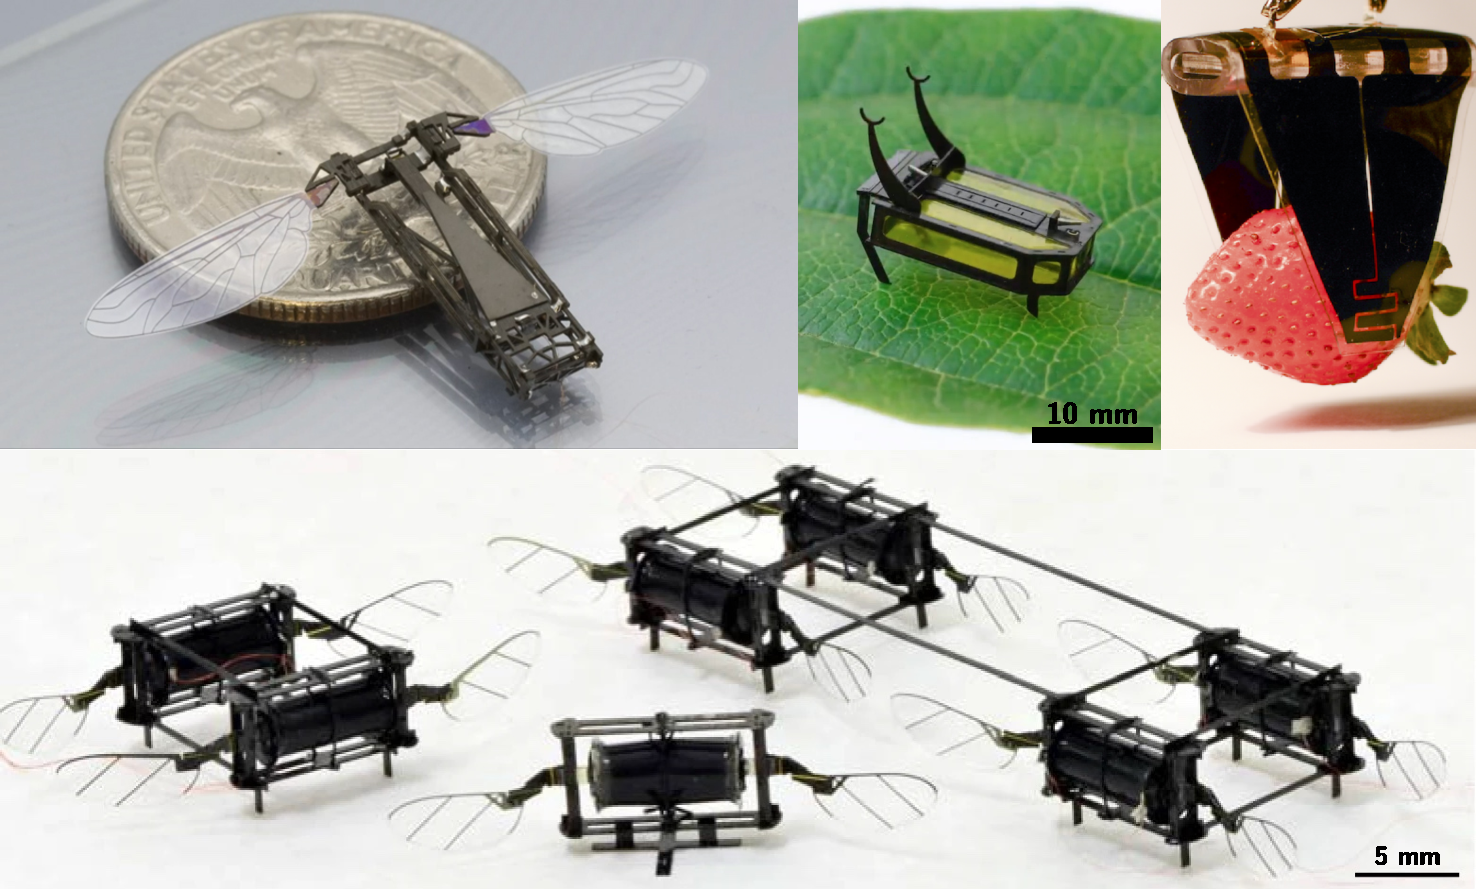
\includegraphics[width=\textwidth]{images/chap0/smart-actuator-examples-small.pdf}};
    % Insert a relative reference based on image dimensions
    \begin{scope}[x={(graph.south east)},y={(graph.north west)}]
        \node [anchor=south] (a) at (0.048,0.51) {\large \textbf{(a)}};
        \node [anchor=south] (b) at (0.57,0.51) {\large \textbf{(b)}};
        \node [anchor=south] (c) at (0.82,0.51) {\large \textbf{(c)}};
        \node [anchor=south] (d) at (0.048,0.4) {\large \textbf{(d)}};
        % \draw[black,ultra thick,rounded corners] (0.62,0.65) rectangle (0.78,0.75);
        % \draw[help lines,xstep=.01,ystep=.05] (0,0) grid (1,1);
        % \foreach \x in {0,1,...,9} { \node [anchor=north] at (\x/10,0) {0.\x}; }
        % \foreach \y in {0,1,...,9} { \node [anchor=east] at (0,\y/10) {0.\y}; }
    \end{scope}
    \end{tikzpicture}%
\end{document}
